\documentclass[../document]{subfiles}

\begin{document}

\section{Sprint 4}

\subsection{Introduction}

The following chapter includes all the documentation regarding the fourth sprint. The fourth sprint will last for eleven days, starting with November 3 and ending on November 14. In this time we will be addressing the new requirements from the customer and we will try to complete all of them in the time that we have. 

\subsection{Sprint planning}

This sprint was not planned to begin with. It is the result of customer requirement after the customer meeting on October 29. The customer was happy with the results of sprint 3, but has expressed some further wishes for the system and pointed out some dislikes. As we are at the end of course, our primary focus is on finishing the documentation. However, since our implementation is modular, we are able to allocate group members and work on par with sprint 4 as well.

There is no direct estimate as to how many of us can work on the implementation of sprint 4. The estimated work hours for this sprint is sixty hours for implementation and forty hours for documentation, making a total of a hundred work hours for the duration of the sprint. This means that on a full workload, four members should be just enough to finish the sprint 4, working at twenty-five hours a week for a total of seventy-five hours. The rest of the group members will work on the documentation pertaining to the entire report, but will be closely involved with the sprints progress, as the sprint will also add new parts of the documentation in the requirements and test plan chapters.

\subsection{Sprint goals}

In this sprint we will have three major goals. The first goal of this sprint is to complete a script that inputs mock-up data. The second goal is to create a system with at least three central hubs, so that we may triangulate the position of the sensors in the environment. The last goal is to implement this into the visualiser while retaining as much modifiability as possible.

As a short list, these are our goals for this sprint:
\begin{enumerate}
	\item
	Create a script that inputs random data into the database.
	\item
	Create a system that can support three or more central hubs, so that we may trilaterate the position of the sensors.
	\item
	Implement the system into the visualiser.
\end{enumerate}

\subsection{Sprint backlog}

\begin{table}[H]
\caption{Sprint Backlog}
\centering
\begin{tabularx}{\textwidth}{|l|X|l|l|l|}
\hline
	Item
	&Task
	&Priority
	&Estimated hours
	&Actual Hours
	\\ \hline 1.1
	&Implement functionality for multiple gateways
	&H
	&10
	&7
	\\ \hline 1.2
	&Implement functionality to support link budget 
	&H
	&10
	&6
	\\ \hline 1.3
	&Implement functionality for moving sensors around using link budget
	&H
	&15
	&5
	\\ \hline 1.4
	&Correct problems and fix bugs in the code
	&H
	&10
	&5
	\\ \hline 2.1
	&Make a mathematical formula for the trilateration of the position using link budget
	&H
	&10
	&6
	\\ \hline 2.2
	&Make a script to input and change sensor data in the database
	&M
	&5
	&5
\\ \hline
\end{tabularx}
\end{table}

\subsection{Sprint backlog evaluation}

As we can see from the backlog, we have managed to finish our implementation ahead of time. We had planned for sixty hours of work, and we have managed to finish everything in thirty-four hours of work. This is mostly due to the highly modifiable code that we had written from the start in order to accommodate change. Furthermore, we were careful with the implementation and therefore did not have too many bugs. Overall, we are satisfied with the time this sprint took, especially since there is a lot of documentation the group needs to write for the final report.

\subsection{Testplan}

\begin{table}[H]
\caption{Test 1}
\centering
\begin{tabularx}{\textwidth}{|l|X|}
	\hline
	Test nr:
	&1
	\\ \hline Requirements:
	&5.3, 5.3.1
	\\ \hline Test name:
	&Random data input
	\\ \hline Environment:
	&Runtime
	\\ \hline Description:
	&A script will put random and complete sensor data into the database to serve as our mock-up data. The mock-up data should be equivalent in scope to the data that could be gathered by the sensors.
	\\ \hline Input:
	&Random dash 7 data input
	\\ \hline Output:
	&The database will have multiple mock-up sensors with their own data
	\\ \hline Acceptance:
	&The dash 7 data input must be correct in it’s scope and it must be stored correctly.
	\\ \hline Result:
	&The data is generated and stored correctly.	
	\\ \hline 
\end{tabularx}
\end{table}

\begin{table}[H]
\caption{Test 2}
\centering
\begin{tabularx}{\textwidth}{|l|X|}
\hline
Test nr:
2
\\ \hline Requirements:
5.1, 5.1.1
\\ \hline Test name:
&Multiple gateways
\\ \hline Environment:
&Design time
\\ \hline Description:
&The system will be able to take in multiple gateways for gathering data from the sensors. The link budget value from each sensor must be present for each gateway.
\\ \hline Input:
&Multiple gateways and the link budget from each sensor to each gateway
\\ \hline Output:
&Database will have multiple gateways and each gateway will read every sensor. All the sensors will have link budgets. This also needs to be shown in the visualiser.  
\\ \hline Acceptance:
&The data is correctly stored and shown.
\\ \hline Result:
&The gateways are created, stored and shown correctly.
\\ \hline 
\end{tabularx}
\end{table}

\begin{table}[H]
\caption{Test 3}
\centering
\begin{tabularx}{\textwidth}{|l|X|}
\hline	
Test nr:
&3
\\ \hline Requirements:
&5.2.1, 5.2.2
\\ \hline Test name:
&Trilateration formula
\\ \hline Environment:
&Design time
\\ \hline Description:
&Find a trilateration formula that will work for multiple gateways and can cope with the accuracy of the link budget.
\\ \hline Input:
&Link budget
\\ \hline Output:
&Position on the screen
\\ \hline Acceptance:
&When the position on the screen reflects where the sensor are on the screen. The position needs to be sufficiently accurate for this test to pass. The accuracy is determined by the group members judgment.
\\ \hline Result:
&The position and movement of sensors reflects the link budget correctly.
\\ \hline 
\end{tabularx}
\end{table}

\begin{table}[H]
\caption{Test 4}
\centering
\begin{tabularx}{\textwidth}{|l|X|}
\hline
Test nr:
&4
\\ \hline Requirements:
&5.2.3, 5.2.4, 5.2.5
\\ \hline Test name:
&Animation by link budget
\\ \hline Environment:
&Runtime
\\ \hline Description:
&By using the link budget from multiple gateways, we will be able to animate the movement of the sensors. The movement depends solely on the link budget towards multiple gateways.
\\ \hline Input:
&Changing link budget
\\ \hline Output:
&Animation of the sensor movement by using the link budget
\\ \hline Acceptance:
&When the animation on the screen reflects where the sensors are on the screen. The position and the animation need to be accurate and smooth for this test to pass. The accuracy and animation quality is determined by the group members judgment.
\\ \hline Result:
&The positional animation is correct and the animation quality is above acceptable according to the group judgment.
\\ \hline 
\end{tabularx}
\end{table}

\begin{table}[H]
\caption{Test 5}
\centering
\begin{tabularx}{\textwidth}{|l|X|}
\hline
Test nr:
&5
\\ \hline Requirements:
&All requirement from 5.1, 5.2 and 5.3
\\ \hline Test name:
&Multiple sensors at the same time
\\ \hline Environment:
&Runtime
\\ \hline Description:
&Multiple sensors should be added to the system at runtime. This should not disrupt the system in any way and they should all be positioned on the screen correctly.
\\ \hline Input:
&Start with multiple active sensors and add more as the program runs
\\ \hline Output:
&Sensor animation on the screen
\\ \hline Acceptance:
&When the sensors are added correctly with no system disruption. The sensors also need to be positioned accurately on the screen. The position will be judged by the group members.
\\ \hline Result:
&Hot join works correctly and the multiple sensors are animated correctly.
\\ \hline 
\end{tabularx}
\end{table}


\subsection{Test results}

The tests have all been positive and provided good results. They have also been useful in uncovering problems and bugs that were fixed afterwards. It should be noted that all of the tests were performed with mock-up data, and as such there should be expectancy that the tests should go well. However, we have tried to simulate real sensor data as closely as possible, so that the system is able to change to a live system without any disruptions or bugs. 

\subsection{Sprint results}

During the sprint we have managed to finish the new requirements listed in \subfullref{requirements_sprint_4} and to fulfill of the tests detailed in the  \subfullref{test_plan_sprint_4}. The system is currently able to take any number of gateways and sensors from the database and arrange them correctly in the visualiser. The sensors are also correctly animated using their link budget as weights. There are some limitations to this system, most notably the use of mock-up data and the testing that used the mock-up data. In theory, our implementation should work for live sensor data, however, we did not have the hardware to test nor implement that solution. Due to our modular implementation, we have had less difficulty than expected, and have finished our implementation in due time.

The screenshots of our system working can be seen in \figref{fig:sprint4_1} and \figref{fig:sprint4_2} . In the first figure, we can see a black background, with a legend on the side and a clock, along with some minor effects, such as blur and bloom to make the visualiser look a bit more stylish. These were all present from the previous implementation of the prototype. What is new is the capability of supporting multiple gateways, and the way the sensors move to these gateways. The sensors no longer orbit a singular gateway, but rather have a mathematical formula that uses the link budget as weights to trilaterate the position in between the gateways. The trilateration works for any amount of gateways, as can be seen in the second figure. The gateways, no matter their number, will be placed in an imaginary circle to create a perfect geometrical shape. This is the perfect positioning of the sensors in a room.

\begin{figure}[H]
\centering
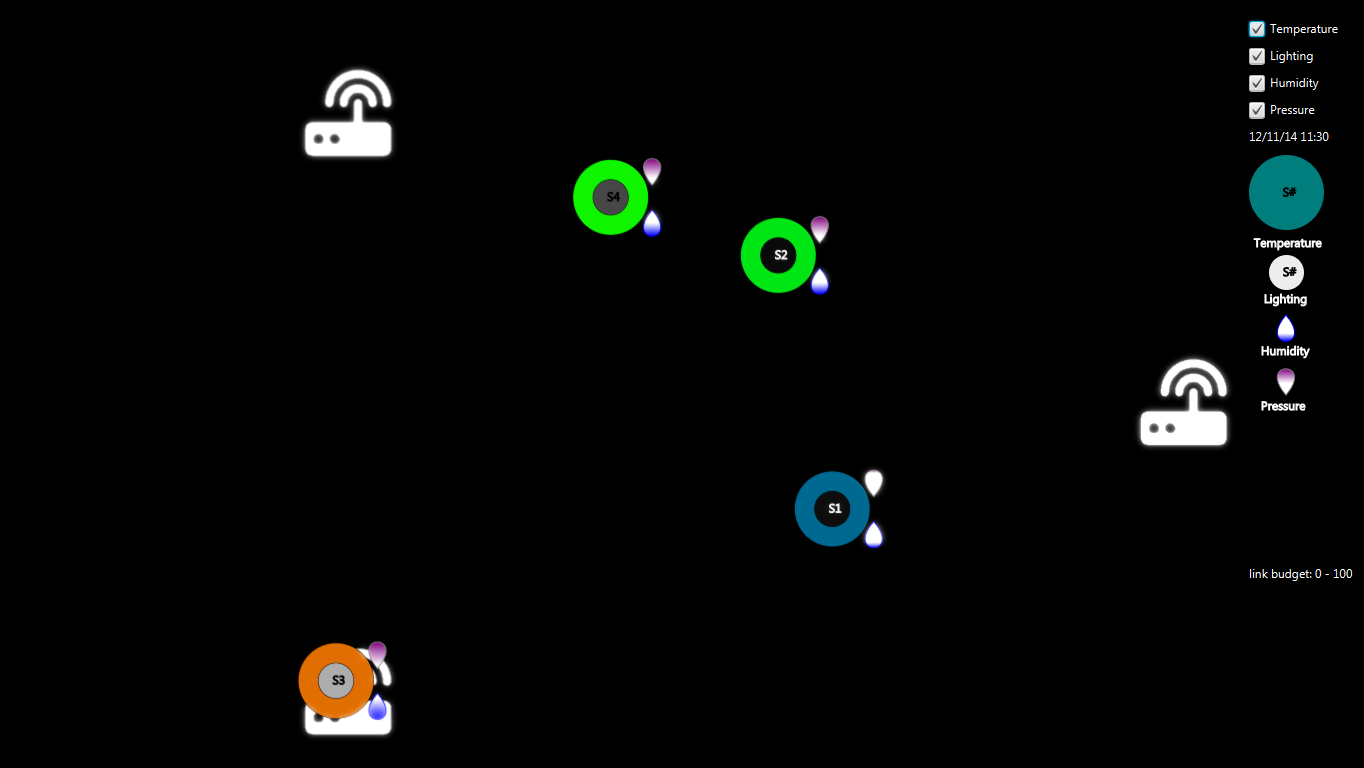
\includegraphics[width=\textwidth]{sprint_4/test_3_gateways.png}
\caption{Sprint 4, 3 gateways}
\label{fig:sprint4_1}
\end{figure}

\begin{figure}[H]
\centering
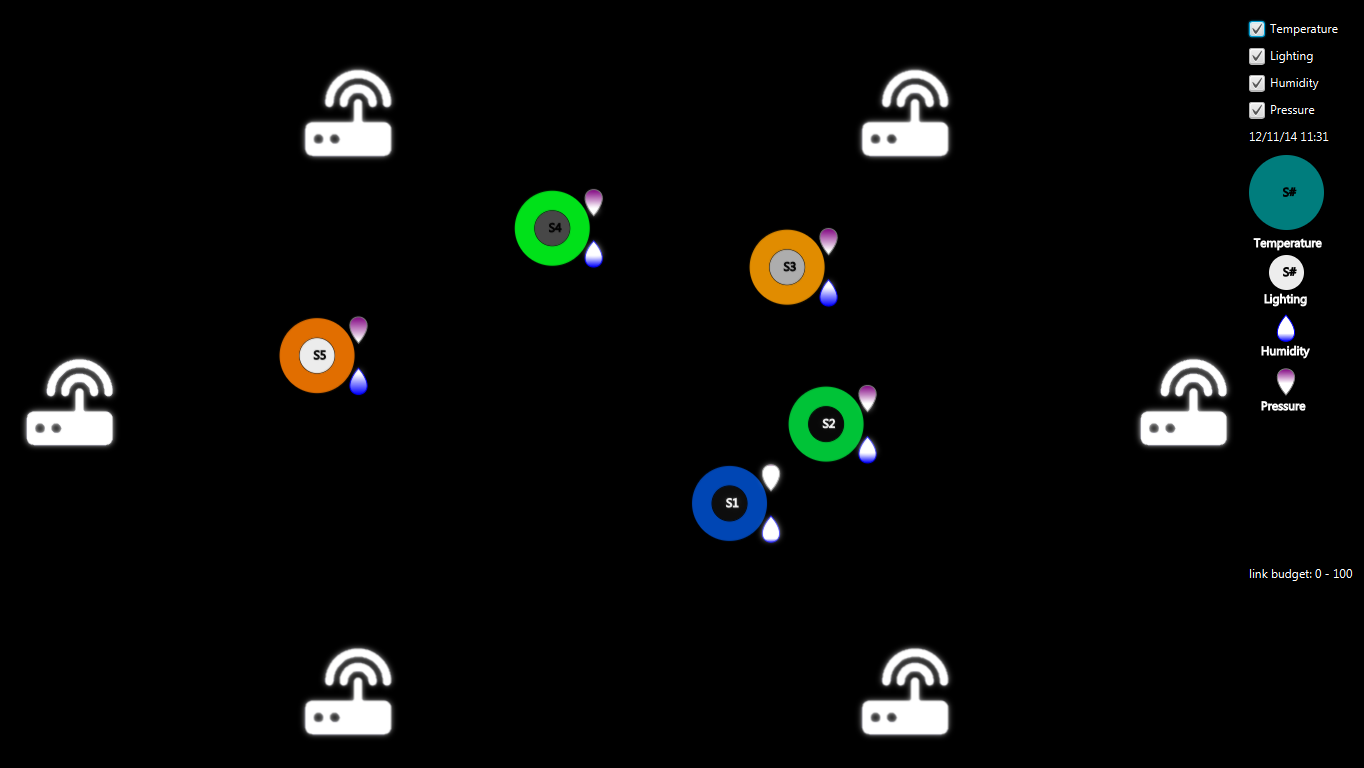
\includegraphics[width=\textwidth]{sprint_4/test_6_gateways.png}
\caption{Sprint 4, 6 gateways}
\label{fig:sprint4_2}
\end{figure}

For sprint 4 it was required that we display data from more than one gateway in the new prototype map view, and that we simulate the environment of two rooms separated by a wall blocking all signals. As the hardware supplied by Altran only included one gateway, it was necessary to develop methods for generation of mock-up data. The main challenge in this was to generate correct link budget data for the different gateways as sensors were moved between the rooms. In addition, we also needed to associate gateways with the correct rooms in both the data generation module and the visualiser module. Several new classes were created to solve the problem, the most important listed below.

\subsubsection{ManualAddDash7Data}
This class allows a user to post DASH7 observations to the database through the console. It has several different modes, most notably a mode that generates and posts data automatically, simulating the multi-room environment. Also included is a manual mode where the user types in all measurement values explicitly, giving the user full control.

\subsubsection{WalledRoomDash7Generator}
This is the class used to simulate the multi-room environment. The constructor of the class needs to be passed a number of parameters, the number of gateways, sensors, and rooms among them. Through the interface the class provides the function nextObservation() from the Dash7Generator interface to generate observations. The link budget of each observation is generated in a pseudo-random fashion, using sensor id, gateway id, and system time as seeds. It also compares the room of the sensor and the gateway; if the rooms are different the link budget is increased, to simulate a decrease in signal strength. Apart from the link budget, the other measurements are generated using as seeds the system time and sensor id only. 

\subsection{Customer review}

During this sprint we met with the customer in the middle of the sprint, rather than at the end of the sprint. This is due to two reasons. First, our time towards the presentation is quite limited, therefore we wanted to know if the customer had any suggestions for the final prototype of the sprint or not, and how satisfied the customer was with the progress. Secondly, we met with the customer earlier because we managed to create a prototype quite quickly, and therefore we had something to show to the customer. We then had a discussion of our upcoming changes, as the prototype was not yet done, and the changes that the customer would like implemented, if time permits. The customer was, overall quite pleased with our progress, and had introduced some changes that we will try to implement until the sprint is finished.

The changes are as follows:
\begin{enumerate}
	\item
	Enable reading from file for link budget calibration. This is a somewhat important change, as we had found out, and the customer later reiterated, that the link budget values typically are measured in between 45 and 100. This was close to our experimentation where we found out that the link budget measurement is in between 40 and 100.
	\item
	Add more gateways if possible, and show the change in simulation from one room to another, and explain what concretely happens in the simulation.
	\item
	It should be possible to monitor the complete path that the data takes, from the sensors to the visualiser.
\end{enumerate}
As far as the last change is concerned, the group agreed that our system already possesses such capabilities. As far as the two other changes are concerned, we will do our best to implement those as well.

Furthermore, this sprint sparked several points of interest where our customer would enjoy our opinion. These include both our findings about the sensors as well as our experience with using mock-up data and real data.

First, we will discuss the use of mock-up data versus real data. The advantage of mock-up data is quite clear; we are able to manipulate the data quickly to test the system. Furthermore, we are able to test the limitations of the system without the need to set up the entire set of sensors and the Raspberry Pi. The main disadvantage of mock-up data is the difficulty of changing it in the database manually. Writing programs that generate data automatically is possible but difficult, especially when simulating an environment where the link budget is affected by walls. The sprint 4 evaluation details our findings regarding automatic data generation further. The main advantage of real-time data is that it is consistently generated. The disadvantage is that the sensors in the current state are not very capable at measuring some values. In our experience, the sensors have problems measuring temperature, humidity and pressure. The measurements of lighting and the accelerometer work well. The link budget, that we were concerned with in this sprint, works to some degree, but was found to be inaccurate. A final disadvantage is that the sensors take some time to set-up.

\begin{table}[H]
\caption{Sprint Results}
\centering
\begin{tabularx}{\textwidth}{|l|X|X|}
\hline
Data Origin
&Pros
&Cons
\\ \hline Real Data
&Consistently generated data.
&Sensors take time to set up. Some measurements are accurate, some measurements are inaccurate.
\\ \hline Mock-Up Data
&Can manipulate the system to generate changes that we want quickly. Quicker testing, and we can test the limitations of the system better.
&Difficult to add or change data consistently.
\\ \hline 
\end{tabularx}
\end{table}	

The next discussion was concerning historical playback. The historical playback was not a high priority, and we have not put much of our implementation effort towards it. However, we do have a system that could, with some work, be used for historical playback quite effectively. What the system does is write to a file. The write to file is identical to the database, and to produce historical playback, one could simply read the program line by line. The writing is implemented, however, reading from the file is not, and the group does not see it as priority. We have, however, submitted this information to the customer, so that it can be used in further development, if necessary.

Link budget was discussed next. We had expressed our concerns before, that the link budget is quite an inaccurate way of measuring the distance of the sensors to the Raspberry Pi, or whichever system of clients and sensors are to be used. Physical objects, like walls, severely increase the link budget. Normally, the link budget is increased by one for every one to two metres. This increase is not quite consistent all the time. When placed behind a physical object, like a wall, the increase in the link budget was an instantaneous ten. Furthermore, going down two flights of stairs increased the link budget further by only five more. The group has therefore concluded that walls and other obstacles should not, if possible, interfere with the sensors and the central hub that collects the sensor information.

Finally, we discussed the preference of mapping and triangulating. Firstly, it should be stated that as there are no angles, the method that we use is trilateration. Secondly, it is more preferable, as we have found out, is to use weights for link budgets rather than any trilateration methods. The reason for this is as follows; when using weights, we include each link budget from each central hub. These link budgets are then summarized and divided. The sensor is then placed in between the central hubs, based on the collective weights of the central hubs. This potentially diminishes accuracies in the system that could come from walls or other objects, but increases the complexity of the system, as it requires more central hubs. However, it is important to note that even with just one parameter, the link budget, it was fairly easy to increase the accuracy, as long as we can increase the number of central hubs in the system. While trilateration was tried (and succeeded) within the sprint, out of the two solutions the group had agreed that the weights are more accurate and work better with the system as is.

\subsection{Sprint evaluation}

We have successfully completed all of the goals in this sprint. The automatic script that we have created is able to generate mock-up data without our intervention, simulating the live data as correctly as possible. While it does not have any usage when the prototype runs with real data, if it could run with real data, it was extremely important for us to finish the script, both for testing and for presentation purposes.

Furthermore, the system is fully implemented with the visualiser. We have made adjustments in how we show multiple gateways, and adjustments in animation, from orbiting to static movement based on link budget. While we do have a limitation of perfect geometrical set-up of gateways in a room, the limitation, we feel, is acceptable in this case. The system is now able to simulate any amount of gateways and sensors in the visualiser.

Finally, we had a discussion with our customer about the sensors and the system overall, and did some more extensive research on the pros and cons of the system. We have learned a lot from this research and will definitely apply more research for future development and topics that we work with. 


\end{document}